\section{Introduction}\label{sec:LoadingAtoms}

After focusing a far-detuned leaser beam to a sufficiently tiny spot (optical tweezer), it was shown that in the presence of resonant light, it is possibly to non-deterministically load the trap with single atoms \cite{Schlosser2001}.
This can be described by an elegant model taking into account one-body as well as two-body loss terms. 
Denoting the average number of atoms in the dipole trap by $N$, time time evolution of $N$ can be described as \cite{Schlosser2002} 

\begin{equation}\label{eq:LoadingTweezer}
	\frac{\text{d}N}{\text{d}t} = \alpha - \gamma N - \beta N(N-1),
\end{equation}
where the first term $\alpha$ is the loading rate or the amount of atoms entering the trap.
Furthermore, $\gamma$ is the atom loss as a result of collisions with the background gas, so this is effectively a one-body loss term.
Lastly, $\gamma$ is a measure for the mainly two-body loss as a result of light-assisted collisions.
In the regime $\beta \gg \gamma$, two-body loss rates are dominant over one-body contributions. 
Because of light assisted-collisions with the help of resonant light, atoms are now kicked out of the trap in pairs.
This will continue until either $N=0$ or $N=1$, where both outcomes have roughly 50\% probability.
This is known as the collisional blockade mechanism \cite{Schlosser2001} or parity projection.

Thus we need to maximize the parameter $\beta$ in \cref{eq:LoadingTweezer}, which can be done by minimizing the trapping volume, the physical size of the optical tweezer.
Additionally, by minimizing the dimensions of the tweezer, less laser power is needed per trap and the traps can be spaced closer together, which is the key to scaling to a higher number of qubits.

There is a fundamental limit to the smallest possible spot size however, which we quantify in \Cref{sec:DiffractionLimit}, where we also elaborate on how to approach this limit in practice.
In \cref{sec:MeasuringTweezer} the setup used to measure the spatial profile of the tweezer is introduced, the results of which are presented along the radial (\cref{sec:TweezerRadial}) and axial (\cref{sec:Tweezer3D}) directions.

\section{Diffraction: Thin Lens}\label{sec:DiffractionLimit}

The basic idea of an optical tweezer is to send a laser beam through a lens.
Because of the wave character of light, there is a fundamental limit to the smallest spot size one can focus this laser beam, even in the absence of aberrations.
Consider a circular lens with aperture radius $R$ and focal length $f$.
We assume it is a thin lens positioned at $z=0$.
The complex light field just before and just after the lens are denoted $E_i(x',y')$ and $E_l(x',y')$ respectively, both for $z=0$.
See \cref{fig:LensAperture}.
The input field $E_i$ used in this work is given in \cref{eq:GaussianAperture}, but can be ignored for now.
We describe the diffraction of the light in the plane after the lens $E(x,y,z)$ in terms of the Fresnel diffraction integral \cite{Goodman2005}

\begin{figure}
	\centering
	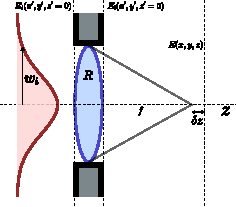
\includegraphics[width=0.6\textwidth]{figures/lens.pdf}
	\caption{Thin lens with aperture radius $R$ and focal length $f$. 
	The input field is $E_i(x',y')$ (\cref{eq:GaussianAperture} which is only within the aperture region. Figure adapted from \cite{Leseleuc2018,Gu2000}.}
	\label{fig:LensAperture}
\end{figure}

\begin{equation}\label{eq:FresnelDiffractionGeneral}
    E(x,y,z) = 
    \frac{e^{ikz}}{i \lambda z} \iint_{-\infty}^{\infty} E_l(x',y') \exp{\left[\frac{ik}{2z}\left((x-x')^2+(y-y')^2\right)\right]} dx'dy'.
\end{equation}
In \cref{eq:FresnelDiffractionGeneral}, $\lambdaup$ is the wavelength and $k=2\pi/\lambdaup$ the wavenumber.
The field after the lens follows from the lens transfer function in terms of the field just before the lens $E_i(x',y')$ as \cite{Goodman2005}

\begin{equation}\label{eq:Transfer}
	E_l(x',y')= E_i(x',y') \exp{
		\left[\frac{-i k}{2 f}(x'^2+y'^2)\right].
	}
\end{equation}
Hidden in the term $E_i(x',y')$ is the aperture function, which is zero for $x'^2+y'^2>R^2$, or in cylindrical coordinates $r>R$.
Inserting \cref{eq:Transfer} in \cref{eq:FresnelDiffractionGeneral} yields after some rearrangement and after omitting the phase-factors in front of the integral, which will disappear when computing the intensity $I=|E|^2$ anyway \cite{Gu2000}

\begin{equation}\label{eq:FresnelDiffracion}
	E(x,y,z) \propto 
	\iint_{-\infty}^{\infty} E_i(x',y')
	\exp{\left[
		\frac{ik}{2}(x'^2+y'^2)\left(\frac{1}{z}-\frac{1}{f}\right)
	\right]}
	\exp{\left[\frac{-ik}{z}\left(xx'+y'y'\right)\right]} dx'dy'.
\end{equation}
Which might look like an impossible integral to solve, which it is usually.
However, in the next sections it will hopefully become clear that for specific cases the integral simplifies greatly.  

\subsection{In the Focus Plane}

A special case of \cref{eq:FresnelDiffracion} is to look only what happens in the focus of the lens, or setting $z=f$.
The tweezer arrays shown in this work are all in the focus plane of this lens, where this condition applies.
Doing this, the integral reduces to 

\begin{equation}\label{eq:FraunhoferDiffractionIntegral}
    E(x, y, z=f)=\iint_{-\infty}^{\infty} E_i(x', y') \exp \left[\frac{-ik}{f}(x x'+y y')\right] dx' dy'.
\end{equation}
which is the Fraunhofer diffraction integral. 
It is the 2D spatial Fourier transform of the 'input' field $E_i$ in $x$ and $y$, with spatial frequencies $f_x = x/\lambdaup f$ and $f_y = y/\lambdaup f$ respectively.
For circular apertures, a description in cylindrical coordinates is more natural however. 
Using the standard definitions for cylindrical coordinates and assuming spherical symmetry (independence of $\theta$), \cref{eq:FraunhoferDiffractionIntegral} can be written as 

\begin{equation}\label{eq:FourierBessel}
	E(r,z=f) \propto 2\pi \int_0^{\infty} E(r') J_0\left( \frac{k r r'}{f}\right) r'dr',
\end{equation}
where we used the definition of the  Bessel function of the first kind of order zero\footnote{$J_0(x) = \frac{1}{2\pi} \int_0^{2\pi} \exp{(i x \cos{\alpha})} d\alpha$, where  $\alpha=\theta-\theta'$.} $J_0(x)$. 
This is the Fourier-Bessel or Hankel transform of the function $E(r')$.
Assuming the beam is Gaussian with 'input' waist $w_i$, the input light field is up to a normalization constant $A$ (see \cref{fig:LensAperture})

\begin{equation}\label{eq:GaussianAperture}
    E(r')=
    \begin{cases}
        A e^{- r'^2/w_i^2},& \text{if } r' < R\\
        0,               & \text{otherwise}.
    \end{cases}
\end{equation}
Substituting \cref{eq:GaussianAperture} in \cref{eq:FourierBessel} yields

\begin{equation}\label{eq:FourierBesselAperture}
    E(r) \propto \int_0^R e^{-r'^2/w_i^2} J_0\left(\frac{k r r'}{f}\right)r'dr'.
\end{equation}
\Cref{eq:FourierBesselAperture} is analytically solvable only for specific cases.
Letting $w_i/R$ go to infinity \cite{Madjarov2020}, which is to treat the incident Gaussian beam as a plane wave, we can neglect the exponential term in \cref{eq:FourierBesselAperture}. 
The integral is now tractable, yielding the field amplitude

\begin{equation}\label{eq:AiryField}
    E(r) \propto \frac{f}{kRr} J_1\left(\frac{k R r}{f}\right).
\end{equation}
Here, the function $J_1$ is the Bessel function of the first kind (order one).
Taking the absolute value squared and normalizing yields the intensity distribution described by the Airy function:

\begin{equation}\label{eq:NormalizedPSF}
    \frac{I}{I_0} = \left[
    \frac{2J_1(k r R/f)}{k r R/f}
    \right]^2.
\end{equation}
Which is plotted in \cref{fig:AiryPlots}.
In 3D, so also considering defocus, the optical response of a perfect lens to this plane wave is known as the \ac{PSF}, which we will use in \cref{sec:Tweezer3D}.
Solving for the first zero of \cref{eq:NormalizedPSF}, and introducing the definition of \ac{NA} of a compound microscope objective: $\text{NA} = R/f$, yields the radius of this Airy disk, which is plotted in \cref{fig:AiryPlots}:

\begin{figure}
    \centering
    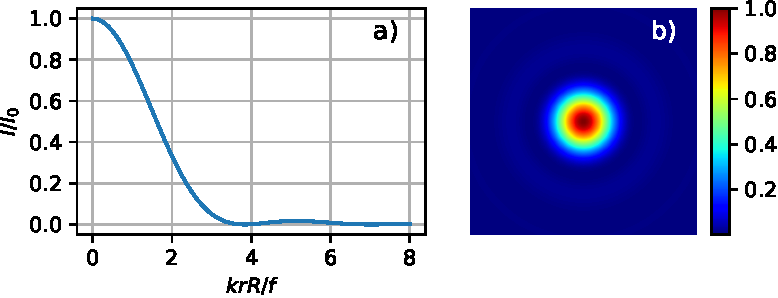
\includegraphics[width = 0.9\linewidth]{figures/AiryDisk.pdf}
    \caption{Normalized plots of the Airy function for \textbf{a)} only the radial coordinate (normalized in units of $k/kR$) as well as \textbf{b)} a 2D plot: the Airy disk.}
    \label{fig:AiryPlots}
\end{figure}

\begin{equation}\label{eq:Abbe}
    d_1 = 0.61 \frac{\lambdaup}{\text{NA}}.
\end{equation}
This result is known as the Abbe limit or diffraction limit \cite{Abbe1882} and it is the smallest feature a lens can produce.
To minimize $d_1$ in \cref{eq:Abbe} we can thus increase the \ac{NA} of our imaging system. 
In this work we will use $\text{NA} = 0.5$\footnote{For high NA imaging systems however, the paraxial approximation which was used to simplify the diffraction integral is no longer a priori applicable. 
Though, \cite{Chon2007} present a derivation of \cref{eq:Abbe} using a different diffraction theory that does not require paraxial approximation and showed that for collimated laser beams \cref{eq:Abbe} has negligible error even for $\text{NA} = 1$. 
We will assume we can still apply \cref{eq:Abbe} for $\text{NA} = 0.5$.}
In practice, it is not convenient to use \cref{eq:FourierBesselAperture} to fit data and it is more convenient to use a simpler function. 
A Gaussian function is commonly used, and can sometimes even fit better than \cref{eq:FourierBesselAperture} because the rings of the Airy disk are easily deformed because of aberrations \cite{Knottnerus2018}. 

\mbox{}\par
\begin{mdframed}
    \subsubsection*{Intermezzo Gaussian Beams}\label{sec:GaussianBeams}
    
    Because we will frequently use the parameters of a Gaussian beam, we will review them here. 
    Starting from Maxwell equations, one can derive under paraxial approximation a description of the transverse electromagnetic mode (TEM\textsubscript{00}) \cite{Leeuwen2017} for the electric field $E$.
    This Gaussian beam is most conveniently written down in cylindrical coordinates $\{r,z\}$:
    
    \begin{equation}\label{eq:GaussianBeam}
    	E(r,z) = \frac{w_0}{w(z)} \exp{\left(\frac{-r^2}{w^2(z)}\right)} \exp{\left[-ikz-i\frac{kr^2}{2R(z)} - i\psi(z)\right]},
    \end{equation}
    with parameters
    
    \begin{equation}\label{eq:GaussianBeamParameters}
    	k = \frac{2\pi}{\lambdaup}, \quad 
    	w(z) = \sqrt{w_0 + \frac{z^2}{z_R^2}}, \quad \text{and} \quad
    	R(z) = z \left(1 + \frac{z^2}{z_R^2}\right).
    \end{equation}
    Respectively, the wave number in terms of the wavelength $\lambdaup$, the beam waist, the radius where the field drops $1/e$ in terms of $w(z)\equiv w_0$ and $R(z)$ is the wavefront curvature. $z_R$ is the Rayleigh range, the distance along the optical axis where the beam waist has increased a factor of $\sqrt{2}$: $w(z=z_R) = \sqrt{2}w_0$.
    Finally $\psi(z)$ is an extra phase term originating from the curvature of the wavefront known as the Gouy phase.
    We find the intensity of the Gaussian beam by taking the absolute value squared:
    
    \begin{equation}\label{eq:GaussianBeamIntensity}
    	I(r,z) = I_0 \frac{w_0^2}{w^2(z)} \exp{\left(\frac{-2r^2}{w^2(z)}\right)}.
    \end{equation}
    A sketch of a Gaussian beam profile is given in \cref{fig:GaussianBeam}, showing the $1/e$ field radius, or $1/e^2$ intensity radius $w_0$ and the Rayleigh range $z_R$. 
    
    \vspace*{3mm}
    \centering
        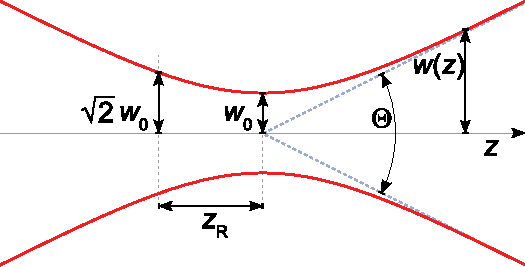
\includegraphics[width=0.52\linewidth]{figures/GaussianBeam.pdf}
        \captionsetup{margin=0mm}%somehow this works
        \captionof{figure}{Gaussian beam profile and some key parameters used in this work, the beam waist $\mathsf{\textit{w}_0}$ and Rayleigh range $z_R$. 
        Figure adapted from \cite{Hermans2009}.}
        \label{fig:GaussianBeam}
\end{mdframed}
Fitting this Gaussian as closely as possible to an Airy function using a least-squares optimization, it can be shown that the equivalent Gaussian waist is \cite{Zhang2007}

\begin{equation}\label{eq:GaussianAiryFit}
    w = 0.42 \frac{\lambdaup}{\text{NA}}.
\end{equation}
This the agreement of this approximation is excellent, but it is only valid near the center region of the Gaussian. 
If our measured waist is at the limit of \cref{eq:GaussianAiryFit}, the tweezer is said to be diffraction limited, that is: the spot size is limited because of the wave character of light and not because of optical aberrations. 
At this point, it is instructive to get a feeling for the spatial profile of the dipole potential.
From \cref{eq:Stark} we know that the potential of the tweezer is proportional to the light intensity. 
Assuming the dipole potential can be described by a Gaussian, which is valid \cite{Zhang2007} near the center of the trap, the potential $U(r,z)$ in cylindrical coordinates is

\begin{equation}\label{eq:GaussianPotential}
    U(r,z)=\frac{-U_{0}}{1+z^{2} / z_{R}^{2}} \exp \left[\frac{-2 r^{2}}{w_{0}^{2}\left(1+z^{2} / z_{R}^{2}\right)}\right],
\end{equation}
where we used \cref{eq:GaussianBeam,eq:GaussianBeamParameters}.
\Cref{eq:GaussianPotential} is plotted in \cref{fig:GaussianPotential} as function of the normalized radial $r/w_0$ and axial $z/z_R$ coordinates. 
The figure is not to scale: the Rayleigh range $z_R$ is typically bigger than the waist $w_0$.
We will use equations of the form \cref{eq:GaussianPotential} to fit optical tweezer potentials.

\begin{figure}
    \centering
    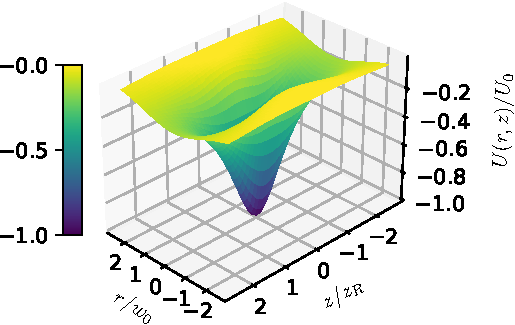
\includegraphics[width=.67\linewidth]{figures/GaussianPotential.pdf}
    \caption{Normalized potential $U/U_0$ for a Gaussian trap shape as a function of the normalized cylindrical coordinates $r/w_0$ and $z/z_R$. Not to scale: typically $z_R > w_0$.}
    \label{fig:GaussianPotential}
\end{figure}

\subsection{Input Beam Size}\label{sec:TweezersPractice}

In producing the perfect \ac{PSF} we assumed plane wave illumination ($w_i \gg R$, but in reality this is impractical: assuming the beam is aligned with the center of the aperture, the fraction of optical power $P/P_0$ transmitted through the aperture as a function of the incident waist $w_i$ is

\begin{equation}\label{eq:fracPowerCircular}
	P/P_0 = 1 - e^{-2w_i^2/R^2},
\end{equation}
which tends to zero for very wide beams (plane waves), which means low power and shallower traps.
On the other hand, the other extreme case is $w_i \ll R$: the waist is much smaller than the aperture and according to \cref{eq:fracPowerCircular} all of the power is transmitted through the aperture.
It can be instructive to have a look at the shape of the resulting light potential: letting the integration boundary of \cref{eq:FourierBesselAperture} run to infinity and using another Hankel transform pair\footnote{$F_0(k) = \int_0^{\infty} e^{-1/2 a^2 r^2} J_0(k r)r dr = \frac{1}{a^2} e^{-\frac{k^2}{2a^2}}$ \cite{Papoulis2981}.} we find 

\begin{equation}\label{eq:GaussianCase}
	U(r) \propto \frac{w_i^2}{2} \exp{\left(\frac{-k^2w_i^2 r^2}{2f^2}\right)},
\end{equation}
which is another Gaussian, but with a modified waist of $\lambdaup f / \pi w_i$.
This modified waist will go up for smaller $w_i$ (Fourier transform property). 
Thus, the input beam size to be used is a compromise between the amount of power transmitted (and thus the depth of the trap), which is maximum for small beam sizes, and the diffraction limit that one can reach and thus the trap dimensions on the other hand. 
The optimum is better understood using the concept trap frequencies, which are the classical oscillation frequencies when occupying the bottom of the potential. 
Using this assumption of only using the center of the potential, we Taylor expand \cref{eq:GaussianPotential} around $(r,z)=(0,0)$ to second order (the first order vanishes) yielding \cite{Muldoon2012}

\begin{equation}\label{eq:ApproximateGaussianPotential}
	U(r,z) \sim -U_0 - 2U_0 \frac{r^2}{w_0^2} - 2U_0 \frac{z^2}{z_R^2}.
\end{equation}
For this harmonic oscillator potential, one can compute the harmonic oscillation frequencies 
\begin{equation}\label{eq:TrapFrequencies}
	\omega_r = 2\left(\frac{U_0}{m w_0^2}\right)^{1/2}, \quad
	\omega_z= \left(\frac{2 U_0}{m z_R^2}\right)^{1/2}.
\end{equation}
Because $z_R > w_0$, the longitudinal oscillation frequency is lower than the radial frequency. 
Optimizing for maximum trap frequencies is useful because from \cref{eq:TrapFrequencies}, higher trap frequencies translate to deeper as well as physically smaller optical dipole potentials.
The optimum $w_i/R$ ratio in terms of maximizing \cref{eq:TrapFrequencies} was found by \cite{Madjarov2021} to be $w_i\sim R$, which we will use for the remainder of this work\footnote{Because trap frequencies can be probed experimentally, they can be used to perform post-corrections on tweezer arrays as well as shown by \cite{Ebadi2021}.}.

\subsection{Outside the Focus Plane}

We have done measurements on the intensity profile outside of the focus as well.
To compare the obtained results to diffraction theory, we have to return to the more general Fresnel diffraction integral \cref{eq:FresnelDiffractionGeneral}, this time in cylindrical coordinates \cite{Gu2000}

\begin{equation}\label{eq:FresnelCylindrical}
	E(r,z) \propto 2\pi
	\int_0^\infty E(r')\exp{\left[\frac{i k r'^2}{2}\left(\frac{1}{f}-\frac{1}{z}\right)\right]}
	J_0\left(\frac{k r'r}{z}\right)r' dr',
\end{equation}
If the amount of focus is $z=f+\delta z$, and $\delta z \ll f$ (the former is on the order of microns while the latter on millimeters), it holds that

\begin{equation}\label{eq:SmallDefocus}
	\frac{1}{f}-\frac{1}{z}\approx
	\frac{\delta z}{f^2}.
\end{equation}
Moreover, we are mainly interested in the intensity distribution along the optical axis $r=0$, for which the contribution of the Bessel function is unity.
Plugging in \cref{eq:FresnelCylindrical} along with \cref{eq:GaussianAperture,eq:SmallDefocus} yields

\begin{equation}
	E(r=0,z) \propto \int_0^R e^{-r'^2/w_i^2} \exp{\left(
		\frac{i k \delta z}{2f^2}r'^2
		\right)} r'dr'.
\end{equation}
Evaluating the integral and taking the absolute value squared yields the intensity distribution $I$ in the axial direction:



\begin{equation}\label{eq:IntensityAxial}
	I(r=0,z) \propto \frac{w_i^4 e^{-R^2/w_i^2}}{2} \left[
	\cosh\left(\frac{R^2}{w_i^2}\right)-\cos\left(\frac{k \delta z R^2}{2f^2}\right)
	\right]
	\left\{
	1+\left(\frac{k\delta z R^2}{2 f^2}\right)^2
	\right\}^{-1}.
\end{equation}
\Cref{eq:IntensityAxial} is plotted in normalized fashion in \cref{fig:PSFvsLongitudinal} for the case of the Gaussian input beam used: $w_i = R$ as well as the case for the plane wave $w_i \gg R$, yielding the \ac{PSF}.
\begin{figure}
	\centering
	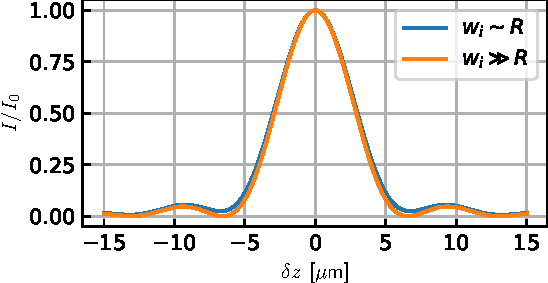
\includegraphics[width=0.68\textwidth]{figures/LongitudinalTweezerField.pdf}
	\caption{Intensity of the tweezer as a function of defocus $\delta z$ along the optical axis for a Gaussian input beam $w_i \sim R$ as well as a plane wave input beam $w_i \gg R$.}
	\label{fig:PSFvsLongitudinal}
\end{figure}
In the latter case, the $\cosh(\cdot)$ contribution in \cref{eq:IntensityAxial} vanishes.
The other numerical values used are the same as in the experiment: $\lambdaup= 820$ nm, $f=4$ mm and $R = \text{NA} \times f = 2$ mm.
From \cref{fig:PSFvsLongitudinal}, the difference between the two cases is small, especially near the focus of the tweezer.





\section{Experimental Implementation}\label{sec:MeasuringTweezer}

From \cref{eq:Abbe}, smallest spot size achieved for the highest numerical aperture, which are typically provided by microscope objectives. 
Apart from high NA, there are other demands on the microscope objective: the \ac{MOT} and subsequent \ac{ODT} are made in a vacuum chamber so the beam traverse a vacuum viewport, requiring:

\begin{enumerate}
	\item Ultra-long working distance (the distance between the trap and the lens). For a single lens, this is equivalent to the focal length $f$.
	For a compound microscope objective however, this does not have to be the case.
	
	\item Glass-thickness compensation. The relatively thick vacuum viewport will introduce a significant amount of aberrations for high NA and therefore large angles. It is possible to correct for this by having additional optics inside of the objective which will pre-correct for this error.
\end{enumerate}

\subsection{Microscope objective}

To satisfy these demands, we chose the G Plan Apo microscope objective from \textit{Mitutoyo}, as also used by \cite{Ebadi2021,Manuel2016}. 
This is an infinity-corrected objective, meaning it is designed to image the projection from its focus to infinity, using an additional field lens to produce an image.
The magnification $M$ the objective and field lens system is in this case 

\begin{equation}\label{eq:InfinityMagnification}
	M = \frac{
		f_{\text{FL}}
	}{
		f_{\text{obj}},
	}
\end{equation}
where $f_{\text{FL}}$ is the focal length of the field lens and $f_{\text{obj}}$ the equivalent focal length of the objective\footnote{For a compound microscope objective, equivalent focal length means the focal length the objective would have when replaced by a single lens.}.
\Cref{eq:InfinityMagnification} is of important when the same lens objective used to produce the optical dipole trap is also used for imaging fluoresence from the same trap.
The infinity-correction has the advantage that it is more flexible than a finite-conjugate corrected objective, as it allows to place additional optics between the laser and the objective without change in alignment.
Additionally, it allows flexible variation of the magnification according to \cref{eq:InfinityMagnification}.
Relevant specifications of the objective for applications in optical tweezers are shown in \cref{table:MitutoyoSpecs}. 
For compound objectives, the equivalent focal length $f_{\text{obj}}$ is defined in terms of the \ac{NA} and the back aperture radius $R$ as $f_{\text{obj}} = R / \text{NA}$, meaning the back aperture radius is 2 mm.

\begin{table}[h]
	\centering
	\caption{Key specifications of the objective from manufacturer Mitutoyo.}
	\label{table:MitutoyoSpecs}
	\begin{tabular}{l | l}
		\textbf{Specification}          & \textbf{Value} \\ \hline 
		NA                              & 0.5            \\ \hline
		Compatible cover glass thickness& 3.5 mm         \\ \hline
		Equivalent focal length         & 4 mm           \\ \hline
		Working distance                & 15.08 mm      
	\end{tabular}
\end{table}
\noindent We measured the transmission for 820 nm laser light for this objective to be $\sim 47$\%, 
Thus quite a significant amount of laser power will be lost. 
We suspect the low transmission is due to the fact that this objective was designed for wavelengths in the visible range, thus all of the lenses inside of it are most likely not anti-reflection coated for 820 nm.

We would like to measure tweezer potential made by our microscope objective to compare to diffraction-limited performance.
We could use time symmetry and look at the reverse direction: using the objective to look at a pinhole, retrieving its \acf{PSF} \cite{Knottnerus2018,Sortais2007}
However, using this method the objective will produce a plane wave, when we know that in practice we do not send a plane wave to the objective(\cref{sec:TweezersPractice}). 
Instead, we used another microscope objective, to look into produced tweezer potential by the \textit{Mitutoyo}. 
In doing this, the tweezer potential will be convolved with the \ac{PSF} of the second microscope objective \cite{Baumgaertner2017}.
Therefore we used a second microscope objective with significantly higher \ac{NA}, minimizing this effect \cite{Baumgaertner2017}. 
However, the Mitutoyo objective is pre-corrected for a piece of glass, e.g. the glass from the glass cell vacuum chamber. 
But this cell is 30 mm thick on the outside, meaning the second objective would also require $\sim 15$ mm working distance which to our knowledge are not available for $\text{NA}>0.5$.
Hence, we use a piece of glass with the same thickness and material (quartz glass, $d = 4.0$) mm to replace one of the walls of the cell, allowing us to look 'into' the cell while minimizing convolution effects.

\subsection{Optical Setup}

The optical setup used for the measurements of this section is shown in \cref{fig:TiSandSLMsetup}. The lower right corner of the figure shows the two objectives and the glass plate. 
The second objective\footnote{Newport M-60X 0.85 NA.} will produce an image onto a linear \ac{CCD} camera\footnote{Point Grey FLEA2 FL2-08S2M.}. 
Because alignment of the Mitutoyo objective with the incident beam, as well as alignment of the two objectives with respect to each other is crucial, both objectives are mounted on 5 axis translation stages.

\begin{figure}
    \centering
    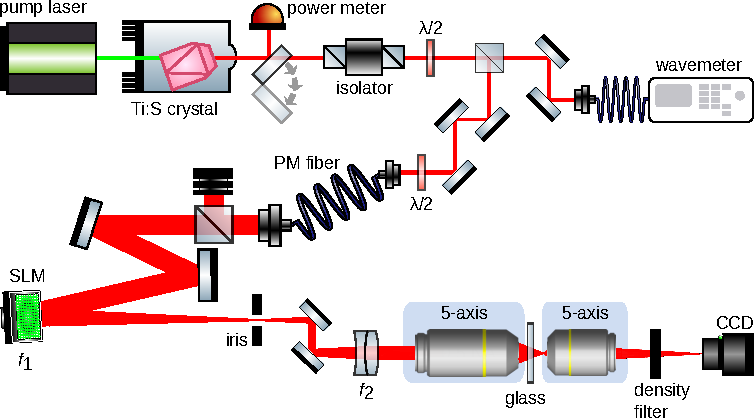
\includegraphics[width=\linewidth]{figures/TiSandSLM.pdf}
    \caption{Output from a titanium sapphire ring laser is coupled into a polarization-maintaining fiber bringing it to the main table. 
    After alignment of the polarization direction, a spatial light modulator $f_1$ and achromatic lens feed the light into the Mitutoyo 0.5 NA objective.
    A glass plate serves to replace the vacuum viewport.
    The tweezer potential is imaged on a camera using a 0.85 NA microscope objective.
    Both objectives are positioned on (piezo) 5-axis stages.
    The cubes shown are polarizing.}
    \label{fig:TiSandSLMsetup}
\end{figure}
On the top of \cref{fig:TiSandSLMsetup} we show the laser source used.
This laser is positioned on a separate table. 
The laser source is a \ac{Ti:S} ring laser\footnote{\textit{Coherent} 899-21 ring laser} (linewidth $\sim 1$ MHz, output power max. $\sim 2$ W.). 
The crystal is pumped using a pump laser\footnote{\textit{Coherent} Verdi V18} (18W power, 532 nm).
The \ac{Ti:S} is easily tunable in wavelength over a wide range. For Sr: 813 nm will be used, but for the experiments for Rb we used 820 nm. 
The reason that we use 820 is that we use a dichroic mirror with a cut-off wavelength of 805 nm to separate the atomic fluorescence from the $D_2$ line at 780 nm from the tweezer light. 
For 820 nm, which is slightly further away from this cut-off than 813 nm, the cut-off performance of this dichroic mirror is better.
Though, the exact wavelength range for Rb is not that important, as long as it is far red-detuned from the atomic transition.

The laser output is brought to the main table using a \ac{PM} optical fiber.
By rotating the $\lambdaup/2$ plate before the PM fiber and aligning the slow/fast axes of the fiber correctly, a constant linear polarization is obtained at the output of the fiber, which is necessary for the \ac{SLM}.
Should the polarization out of the fiber be incorrect however, the incorrect component will be filtered out by a polarizing beam splitter cube, such that the beam to the SLM will always be vertically polarized.
To fully illuminate the SLM, which has dimensions of $\sim 15.4 \times 9.6$ mm (\cref{table:SLMspecs}), a fiber collimator\footnote{\textit{Schäfter + Kirchhoff} 60FC-L-0-M60-10.} with a clear aperture of 17 mm was used ($f=60$ mm, $M^2 < 1.05$, $1/e^2$ beam radius 4.9 mm).
The collimation setting was adjusted for 820 nm by adjusting the lens position in the collimator.

The SLM is more elaborately explained in \cref{ch:arrays}, but a feature worth mentioning here is that the SLM acts as one of the lenses of a telescope, such that the beam traveling to the microscope objective is demagnified by a factor $f_2/f_1$.
The relay lens, $f_2=300$ mm is an achromatic lens in order to minimize aberrations.
The equivalent focal length of the SLM is $\sim 690$ mm, such that $f_2/f_1 \sim 0.42$.


\subsection{Calibration Imaging System}\label{subsec:CameraCalibration}

The 60X magnification of the 0.85 NA objective is only specified when used in a microscope with standard tube length distance, because it is finite conjugate corrected.
Outside of a standard microscope, we have to calibrate its exact magnification.
We do this using a high resolution target\footnote{Technologie Manufaktur TC-RT01}, featuring groups of lines with variable spacing between them. 
The way this was done is shown in \cref{fig:SetupResolutionTarget}.
Initially, we tried to use laser light to illuminate the target, but we did not get a clear image. 
Most likely this is because of the diffracting beams interfering with each other. 
To combat this we used light from an incoherent light source (\ac{LED}). 
We neglect the slightly different focus point from the Newport objective for our laser frequency compared to white light. 
An image of the calibration target showing the spaced lines is shown in \cref{fig:resolutionTarget}.

\begin{figure}
	\begin{subfigure}{.5\textwidth}
	    \flushleft
	    
\includegraphics[height=1.44cm]{figures/white.jpeg}
	    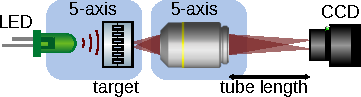
\includegraphics[width=\linewidth]{figures/LEDcalibration.pdf}
	    
\includegraphics[height=1.44cm]{figures/white.jpeg}
		\caption{}
		\label{fig:SetupResolutionTarget}
	\end{subfigure}
	\hfill
	\begin{subfigure}{.45\textwidth}
	    \flushright
		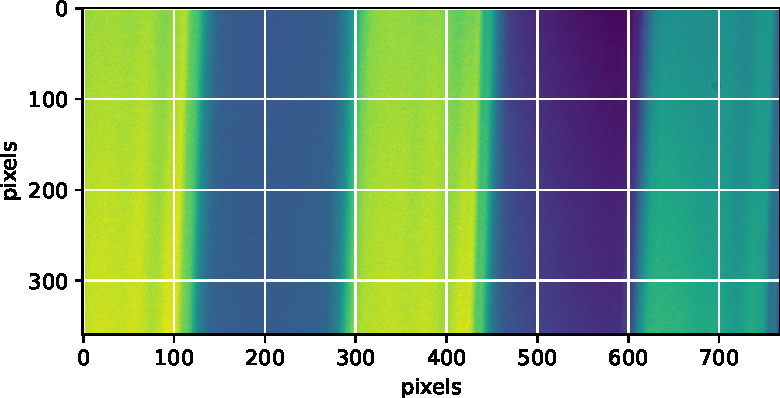
\includegraphics[width=\linewidth]{figures/LineSpacingCalibration.pdf}
		\caption{}
		\label{fig:3Dwaistfit}
	\end{subfigure}
	\caption{\textbf{a)} Illumination of the calibration target by an LED, imaged by the 0.85 NA objective and camera at fixed distance.
	\textbf{ b)} Image from the resolution target illuminated showing lines spaced by 45 lines per mm.}
	\label{fig:resolutionTarget}
\end{figure}

To detect the edges in \cref{fig:resolutionTarget}, we use an edge detection algorithm script.
For several 1D row slices of the image, it blurs the edge using a Gaussian to suppress noise and subsequently computes the spatial derivative. 
When the derivative surpasses a set threshold we define it as an edge.
Dividing the pixel spacing of the lines by the pixel pitch of the camera ($4.65$ $\mu$m) we find a magnification of ($67 \pm 3$)X, which is larger than the 60X specified by the manufacturer. 
The error is a width of the lines, which varied quite a lot with the exact focus distance. 
This is probably because the depth of focus of the 0.85 NA objective is smaller than the thickness of the target. 
We attribute this to a tube length used (objective - camera distance) that was slightly too long.
After the calibration was performed the calibration target was removed and the setup in \cref{fig:TiSandSLMsetup} was used again, the objective-camera distance was kept constant for the remainder of the measurements.

\section{Radial Intensity Distribution}\label{sec:TweezerRadial}

An image of the tweezer at the point of maximum intensity imaged onto a camera through the 0.85 NA objective is shown in fig. \ref{fig:2Dresults}a. 
\begin{figure}
    \centering
    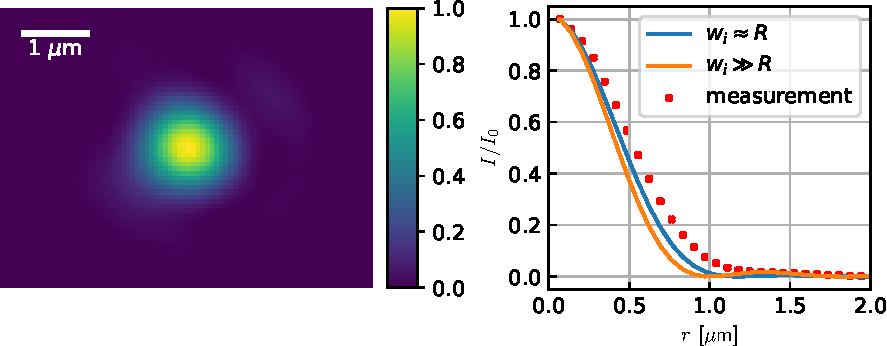
\includegraphics[width=\linewidth]{figures/AzimuthalAverageSpotZoomed.pdf}
    \caption{\textbf{a)} Tweezer as imaged by the second objective onto the CCD camera. 
	\textbf{ b)} Azimuthal average (red) plotted against the ideal \ac{PSF}, \cref{eq:NormalizedPSF} of the objective as well as the result from diffraction theory \cref{eq:FourierBesselAperture} for the input waist used.}
    \label{fig:2Dresults}
\end{figure}
The Airy ring is somewhat asymmetric, suggesting a slight tilt aberration is present.
This slight tilt is difficult to eliminate, as the alignment of the beam with the two objectives, glass plate and camera cannot be independently adjusted: tilting the first objective for example, will change the alignment of the incoming beam as well as the alignment with the glass plate and second objective.
Thus, the aberration could be a result of the imaging onto the camera and not from the potential itself.
In \cref{fig:2Dresults}, an aberration correction using the \ac{SLM} was already applied, which is explained in \cref{subsec:AberrationCorrection}. 
Though, this correction did not have a noticeable effect on the radial distributions shown in \cref{fig:2Dresults}.
There was an effect on the axial distribution however, which is elaborated upon in \cref{sec:Tweezer3D}.

Returning our attention back to fig. \ref{fig:2Dresults}a, we computed an azimuthal average of the radial intensity distribution which is shown in fig. \ref{fig:2Dresults}b.
This was done by integrating the amount of pixel counts in 'rings' around the center pixel.
The rings have a width of 1 pixel, such that the intensity as a function of the distance to the center in pixels can be computed using this binning method.
Distances in pixels were converted to microns using the calibration as described in \cref{subsec:CameraCalibration}.
The measurement is compared against the Airy function or the ideal \ac{PSF} of the objective \cref{eq:NormalizedPSF} when using a uniform input beam, as well as the result from scalar diffraction theory using a Gaussian input beam equal to the aperture $w_i \sim R$, which was used to obtain the measurements.
The latter theoretical result was obtained by integrating \cref{eq:FourierBesselAperture} as a function of the radial coordinate $r$.
From \ref{fig:2Dresults}b, the Gaussian input beam results in a slightly ($\sim 9\%$) broader spot.
Additionally, the rings of the Airy disk will be slightly suppressed, this effect is known as Gaussian apodization.


Comparing the measurement to the theory result, the measurement has a waist which is about $\sim 10\%$ broader. 
The apodization effect is not that clearly visible, possibly because of a slight aberration, which the Airy rings are quite sensitive to.
Possibly, the slightly larger waist is a result of convolution of the tweezer with the \ac{PSF} of the imaging system (see \cref{eq:Deconvolution}. Though the second objective has a significantly higher NA, the convolution effect can have significant contribution.

To check if this is indeed the case, a more accurate analysis method is needed.
For example: in the previous binning method, the exact center location is not determined: it could lie anywhere in the center pixel. 
Also, information is lost during the binning. 
Therefore we also perform a two-dimensional fit using a normalized Gaussian $G/G_0$ in Cartesian coordinates (eq. \ref{eq:GaussianBeamIntensity})

\begin{equation}\label{eq:2DGaussian}
    \frac{G(x,y)}{G_0} =  
    \exp{\left[ -\frac{(x-x_0)^2}{2\sigma_x^2}\right]}
    \exp{\left[ -\frac{(y-x_0)^2}{2\sigma_y^2}\right]}.
\end{equation}
The result of this fit is shown in \cref{fig:3Dshowing}. 
Clearly, the obtained tweezer potential fits very well to a Gaussian, which justifies the assumption of using a Gaussian approximation to estimate the trap frequencies (\cref{eq:GaussianPotential}. 
This is confirmed by the coefficient of determination $R^2 > 0.99$.

\begin{figure}
\centering
	\begin{subfigure}{.49\textwidth}
	    \centering
		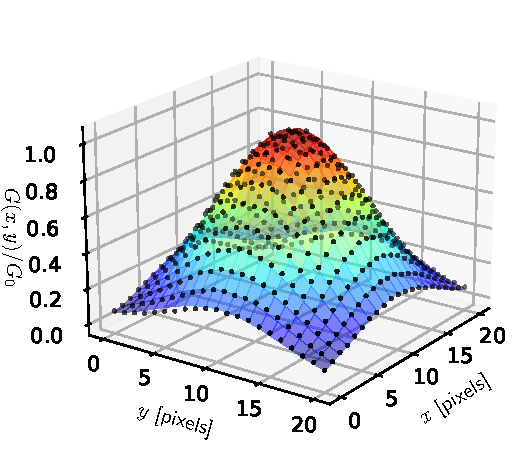
\includegraphics[width=0.96\linewidth]{figures/3DSpotFitGaussian.pdf}
		\caption{}
		\label{fig:3Dshowing}
	\end{subfigure}
	\begin{subfigure}{.49\textwidth}
		\centering
		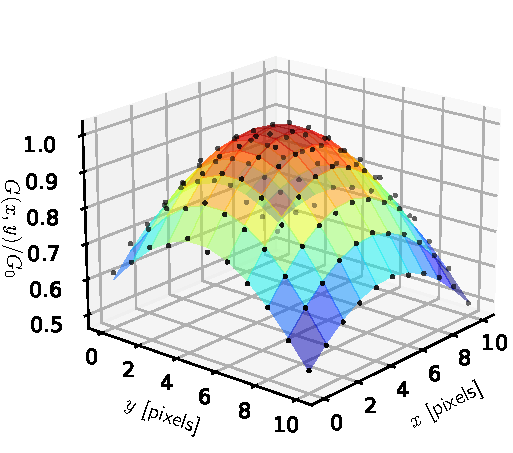
\includegraphics[width=0.96\linewidth]{figures/3DSpotFitGaussianSmaller.pdf}
		\caption{}
		\label{fig:3Dwaistfit}
	\end{subfigure}
	\caption{\textbf{a)} Measured tweezer potential on the CCD camera, as well as the 2D Gaussian fit.
	\textbf{b)} Region of interest around the maximum that was used to extract the waist. For both plots: $R^2>0.99$, but it is higher for the fit in \textbf{b}.}
	\label{fig:3Dfits}
\end{figure}

In order to extract the waist from \cref{fig:3Dshowing}, only the center $10 \times 10$ pixel area was considered as the Gaussian approximation works best for small $r$. 
This was confirmed by the correlation coefficient which was indeed higher for smaller for the fit on the smaller region of interest. 
The result of this fit is shown in \cref{fig:3Dwaistfit}.
Assuming the $\sigma_x \sim \sigma_y$ which should be valid for a circular aperture, we find the waist as $w_{\text{image}} = 2\sigma = \sigma_x + \sigma_y = (0.90 \pm 0.04)$ $\mu$m, where the error originates mainly from the calibration of the magnification. 
Despite the 0.85 NA used, there will still be a slight convolution with the imaging point spread function present. 
Although in deconvolution is non-trivial in general, for the specific case of a Gaussian function, the deconvolved waist $w_{\text{object}}$ can be found in terms of the waists of the image $w_{\text{image}}$ and the diffraction-limited waist of the imaging system $w_{\text{system}}$ according to \cite{Knottnerus2018}

\begin{equation}\label{eq:Deconvolution}
    w_{\text{object}} = \sqrt{w_{\text{image}}^2-w_{\text{system}}^2}.
\end{equation}
This yields $w_{\text{object}} = (0.79 \pm 0.05)$ $\mu$m. 
Comparing to the theory result, for $\lambdaup = 820$ nm and $\text{NA} = 0.5$ (\cref{eq:Abbe,eq:GaussianAiryFit}) yields $w_0 = 0.689$ $\mu$m. 
But this result not possible because of using input beam size $w_i \sim R$. 
We know that as a result of this, the waist should be $\approx$ 9-10\% larger \cite{Chon2007,Sortais2007} which was confirmed by \cref{eq:FourierBesselAperture}, yielding $w_0 \sim 0.75$ $\mu$m, which is in good agreement with the measured result.
We conclude the spot size of the tweezer is nearly diffraction-limited.

\section{Axial Intensity Distribution}\label{sec:Tweezer3D}

To obtain tweezers with the smallest possible volume in order to load single atoms, not only the radial dependency on the intensity distribution is important, but the axial distribution as well.
The relevant parameter here is the Rayleigh range (see \cref{fig:GaussianBeam}).
To study the axial direction, we scan the Mitutoyo objective along the optical axis $z$ using a motorized stage and record an image of the radial profile of the tweezer for each step.
The relevant part of the optical setup for this is shown in \cref{fig:ZScanSetup}.
In the end, all images are stitched together to make a single image that would give an idea of a side view of the tweezer.

\begin{figure}
    \centering
    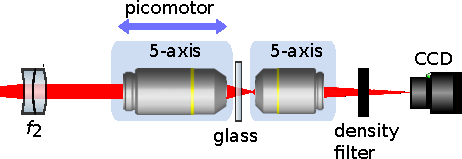
\includegraphics[width=0.6\linewidth]{figures/ZScanSetup.pdf}
    \caption{Optical setup for determining the axial dimension of the tweezer potential. The first objective was scanned along the optical axis using a piezo linear translation stage.}
    \label{fig:ZScanSetup}
\end{figure}


\subsection{Piezo Stage Calibration}

The stage we used is 8081-M 5-axis motorized tilt aligner from Newport. 
Nano-positioning piezo actuators are excellent at producing minuscule ($<30$ nm) step sizes in a repeatable fashion, making them extremely useful for this measurement.
Because of the 5 degrees of freedom, it can accurately align the two objectives with each other. 
To drive this stage, we used a set of Newport 8742 controllers in daisy-chain configuration: both can drive 4 motors so we have 2 of them to address all 5 motors using a set of 8725 multi-axis adapters.
For scanning the axial direction of the tweezer we only use one of the five motors in the stage. 
To know the exact step size calibration is needed because the step size is dependent on the torque applied and the direction of travel.
In order to do this, we repeatedly measured the available translation range of some $\sim$ 3mm, recording the amount of steps this takes as well as the amount moved using a caliper. 
We found a step calibration of $10.6 \pm 0.3$ $\mu$m/step.
The error is a result of uncertainty in the caliper measurements. 



\subsection{Results: Axial Dependency}

\begin{figure}[t]
\centering
	\begin{subfigure}{.49\textwidth}
	    \flushleft
		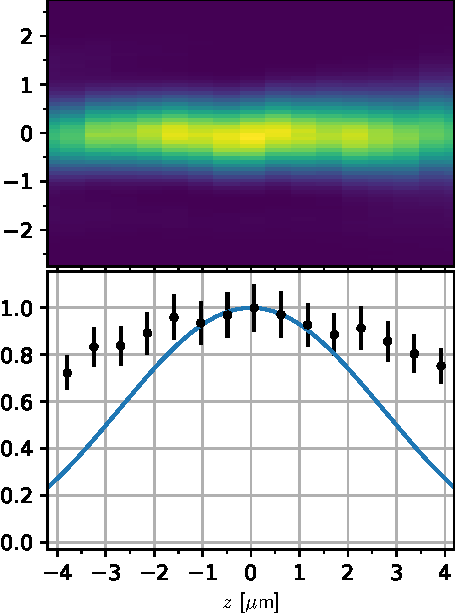
\includegraphics[height=9.5cm]{figures/AxialImageTweezerScanUncorrected.pdf}
		\caption{}
		\label{fig:AxialUncorrected}
	\end{subfigure}
	\begin{subfigure}{.49\textwidth}
		\flushright
		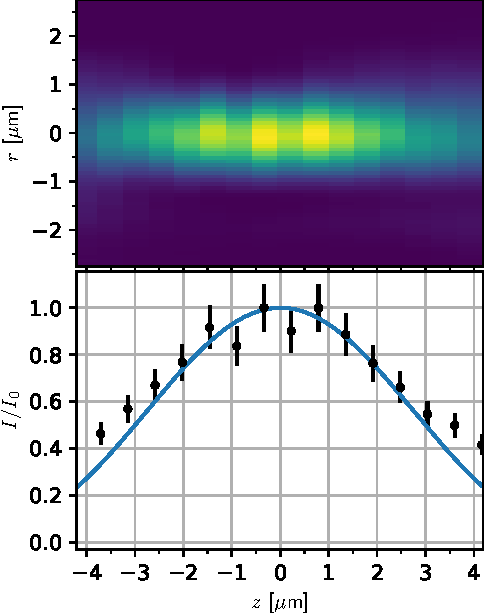
\includegraphics[height=9.5cm]{figures/AxialImageTweezerScan.pdf}
		\caption{}
		\label{fig:AxialZernike}
	\end{subfigure}
	\caption{Radial intensity profile \textbf{a)} prior to aberration correction and \textbf{b)} after aberration correction.
	Also shown: on-axis intensity data as well as the result from theory \cref{eq:IntensityAxial}.
	The error bars are relative errors, mainly from fluctuations in laser intensity.}
	\label{fig:AxialScans}
\end{figure}

In \cref{fig:AxialUncorrected} the scanned profile of the tweezer is shown, as well as the maximum intensity recorded as a function of the amount of defocus $\delta z$ from the center of the tweezer.
The scale is the same in $r$ and $z$ directions, so the aspect ratio is unity.
The error bars are mainly a consequence of fluctuations in laser intensity as well as uncertainty in the piezo stage calibration.
Also plotted is the result from diffraction theory for the case $w_i =R$ from \cref{eq:IntensityAxial}.

Clearly, there is a discrepancy between the theory and measurement results.
This is confirmed by fitting the data to a Gaussian, which was done for the region $(-4, 4)$ $\mu$m of defocus, yielding $z_R \sim 6.2$ $\mu$m, while the diffraction-limited $z_R$ from \cref{eq:IntensityAxial} is $\sim 3.0$ $\mu$m.
We initially attributed the difference to the incorrect glass thickness used: the glass cell and corresponding glass plate consists of 4.0 mm thick quartz glass ($n=1.44$), whereas the cover glass correction of the objective was originally designed for 3.5 mm of N-BK7 glass ($n=1.51$).
The optical thickness $nd$ is thus 0.5 mm larger than the objective is corrected for. 
\begin{figure}[]
    \centering
    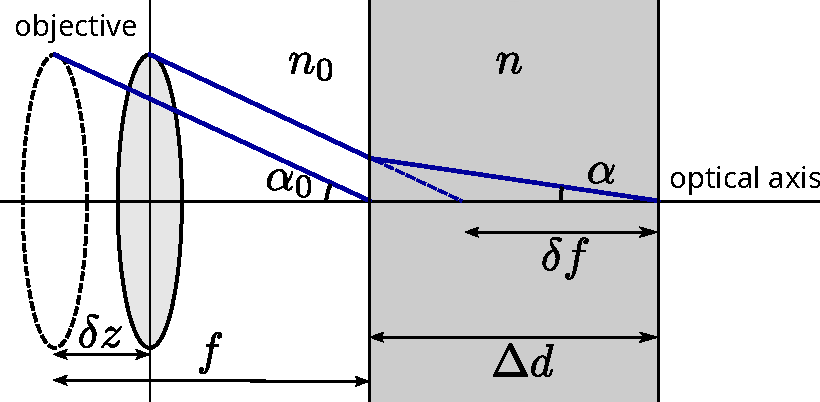
\includegraphics[width=0.55\linewidth]{figures/sphericalAberration.pdf}
    \caption{As a result of extra glass thickness $n\Delta d$, the objective will have to move a distance $\delta z$, corresponding to a change in focus distance $\delta f$.
    The other parameters are explained in the text.
    Figure adapted from \cite{Iwaniuk2011}.}
    \label{fig:SphericalSketch}
\end{figure}
This excess thickness $\Delta d$ is shown in gray in \cref{fig:SphericalSketch} and has refractive index $n$ whereas the surrounding air has $n_0$ which is assumed to be unity.
To simplify geometry, the extra glass is positioned near the focus, but the results are indifferent with respect to the axial location of the glass.
The maximum ray angle is $\sin{\alpha_0} = R/f$. 
Because of the extra glass, the objective is moved an amount $\delta z$ to be in focus.
After some geometry \cite{Iwaniuk2011} this leads to a change in focus $\delta f$:

\begin{equation}\label{eq:SphericalFocus}
    \delta f = \Delta d - \delta z = \Delta d \left[
    1 - \frac{n_r}{\sqrt{1+(1-n_r^2)\tan^2{\alpha_0}}}
    \right],
\end{equation}
where $n_r=n_0/n\approx1/n$ is the ratio of refractive indices and $\tan{\alpha_0} = r/f$ is the incident angle. 
So \cref{eq:SphericalFocus} is a function of $r$ and will not be the same for paraxial rays compared to rays having a larger incident angle (marginal rays). 
In \cref{subsec:AberrationCorrection} we explain how we computed the corresponding phase error of \cref{eq:SphericalFocus}, which we corrected using the \ac{SLM}.
After correction, we measured a reduced Rayleigh range of $z_R \sim 5.2$ $\mu$m, which is still significantly larger than the result from theory. 
Subsequently, we applied an extra cylindrical lens to the SLM to correct astigmatism, which is also explained in \cref{subsec:AberrationCorrection}, yielding a fit of $z_R \sim (3.5 \pm 0.3)$ $\mu$m which is much closer to the $\sim 3.0$ $\mu$m theoretically possible.
This measurement is shown in \cref{fig:AxialZernike}.
The axial intensity distribution is thus not diffraction-limited. 
Most likely, this is caused by an aberration, e.g. a slight tilt in the glass plate or another optical component.




















